\begin{refsection}[research/maruyama/group.bib]
\nocite{*}
\chapter{HPC Programming Framework Research Team}

\section{Members}

\begin{itemize}
  \item[] Naoya Maruyama (Team Leader)
  \item[] Motohiko Matsuda (Research Scientist)
  \item[] Shinichiro Takizawa (Research Scientist)
  \item[] Mohamed Wahib (Postdoctoral Researcher)
  \item[] Keisuke Fukuda (Research Associate)
  \item[] Koji Ueno (Student Trainee)
  \item[] An Huynh (Student Trainee)
  \item[] Satoshi Matsuoka (Senior Visiting Scientist)
  \item[] Tomoko Nakashima (Assistant)
  \item[] Aya Motohashi (Assistant)
\end{itemize}

Text for research Results and achievements. Journal-artcile~\cite{sample-journal}.
Conference-paper~\cite{sample-conference}.
Invited-talk~\cite{sample-invited}.

For cross referencing, use \verb|\locallabel| and \verb|\localref| to avoid conflicting names defined by other groups. For example, a figure can be referenced as Figure~\localref{fig:sample-label1}.

\begin{figure}
\centering
  
\includegraphics[width=0.5\textwidth,keepaspectratio,natwidth=193,natheight=40]
  {sample_division/sample_group/test1.png}
  \caption{Caption for a sample figure}
  \locallabel{fig:sample-label1}
\end{figure}

\section{Research Activities}

We develop high performance, highly productive software stacks that aim to simplify development of highly optimized, fault-tolerant computational science applications on current and future supercomputers, notably the K computer. Our current focus of work includes large-scale data processing, heterogeneous computing, and fault tolerance. A major ongoing project in our group will deliver a MapReduce runtime that is highly optimized for the intra- and inter-node architectures of the K computer as well as its peta-scale hierarchical storage systems. Another major project focuses on performance and productivity in large-scale heterogeneous systems. We also study high performance graph analytics on the K computer. Below is a brief summary of each project.

\section{Research Results and Achievements}

\subsection{KMR}
% Takizawa & Matsuda

\subsection{High Level Framework for High Performance AMR}
% Wahib

\textbf{Summary:}
Adaptive Mesh Refinement methods reduce computational requirements of problems by increasing resolution for only areas of interest. However, in practice, efficient AMR implementations are difficult considering that the mesh hierarchy management must be optimized for the underlying hardware. Architecture complexity of GPUs can render efficient AMR to be particularity challenging in GPU-accelerated supercomputers. In this project, we present a high-level framework that can automatically transform serial uniform mesh code annotated by the user into parallel adaptive mesh code optimized for GPU-accelerated clusters. We show experimental results on three production applications. The speedups of code generated by our framework are comparable to hand-written AMR code while achieving good and weak scaling up to 1000 GPUs.

\textbf{Motivation:}
Frameworks that provide support for GPU in AMR applications~\cite{Parker2006} require the programmer to write his own versions of the target-optimized solvers. Moreover, there can be scalability limitations caused by the overhead of the CPU-GPU communication schemes in those frameworks. We present a high-level framework that specializes in enabling efficient and scalable structured AMR solutions to scientific applications running on GPU-accelerated systems~\cite{Wahib2015}. Our framework uses a high-level programming model that provides an architecture-neutral programming interface and adopts an AMR strategy that would eliminate any CPU-GPU communication schemes that can limit scalability. We base our framework on octree-based AMR implementation in which we use a distributed tree~\cite{Burstedde2011} and adapt the mesh in a parallel fashion with minimum inter-node communication. We base our GPU implementation on a data-centric approach at which the CPU is specialized in managing the data structures representing the mesh hierarchy, while AMR-specific routines that operate on mesh application data are executed on the GPU. Hence keeping the mesh application data arrays on the GPU memory for the entirety of the simulation.

\textbf{Programming model:}
The programming model is designed to be exposed in an architecture-neutral manner; the programmer has no knowledge of the underlying architecture. We provide the programmer with a set of C language directives to identify the stencil functions and data arrays in a logically fixed and uniform mesh implementation of solver(s). The programming interface enables the underlying compiler-based framework to statically analyze the solvers, construct the adaptive mesh hierarchy, automatically parallelize the mesh partition over distributed memory, and apply optimizations required for keeping the mesh application data, i.e., stencil arrays, in GPU memory throughout the simulation. 

\textbf{Optimizations:}
When an AMR code generated by our framework is executed on a GPU-accelerated cluster, the stencil and mesh adaptation kernels run on the GPU, while managing the octree data structures and load balancing is done on the CPU side. Since we pursue efficiency and scalability, code on both the CPU and GPU should be optimized. The stencil kernel and mesh adaptation kernels are memory-bound kernels that are optimized to use the shared memory of the GPU and maintain coalesced memory accesses. For load balancing, \emph{intra-node} load balancing is applied by moving balancing the number of blocks equally among the GPUs. For the \emph{inter-node} load balancing, we rely on a space fitting curve to decide on how to redistribute the blocks.
\begin{figure*}[t]
\centering
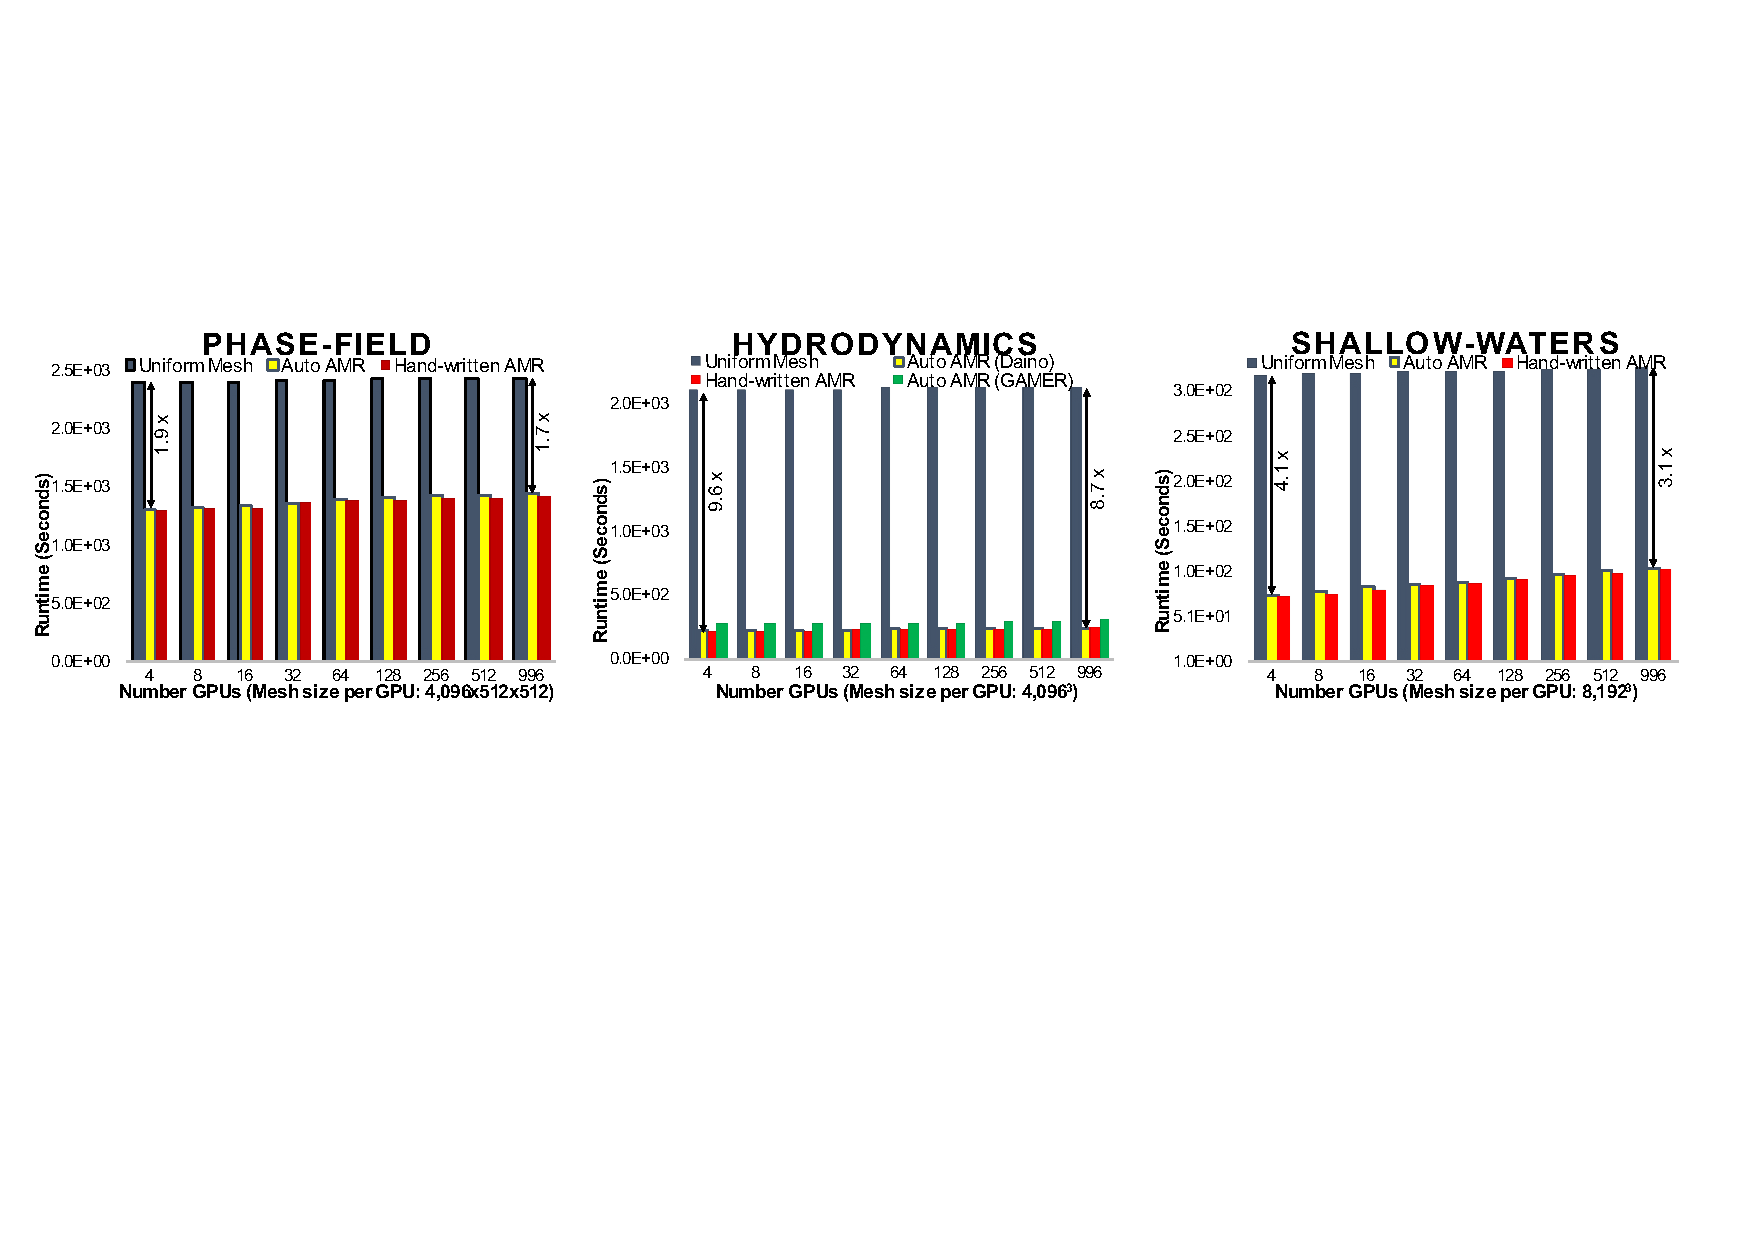
\includegraphics[width=\textwidth]{research/maruyama/wahib01.pdf}%1-expanded.pdf}%1.pdf}, 
%\caption{Weak scaling of hand-written AMR and Daino-generated AMR versus uniform mesh (Note: GAMER-generated AMR included in hydrodynamic solver)}
\caption{\small{Weak scaling of uniform mesh, hand-written and automated AMR (GAMER-generated AMR included in hydrodynamic)}}
  \locallabel{fig:wahib01}
%%\vspace{-5pt}
\end{figure*}
\begin{figure*}[t]
\centering
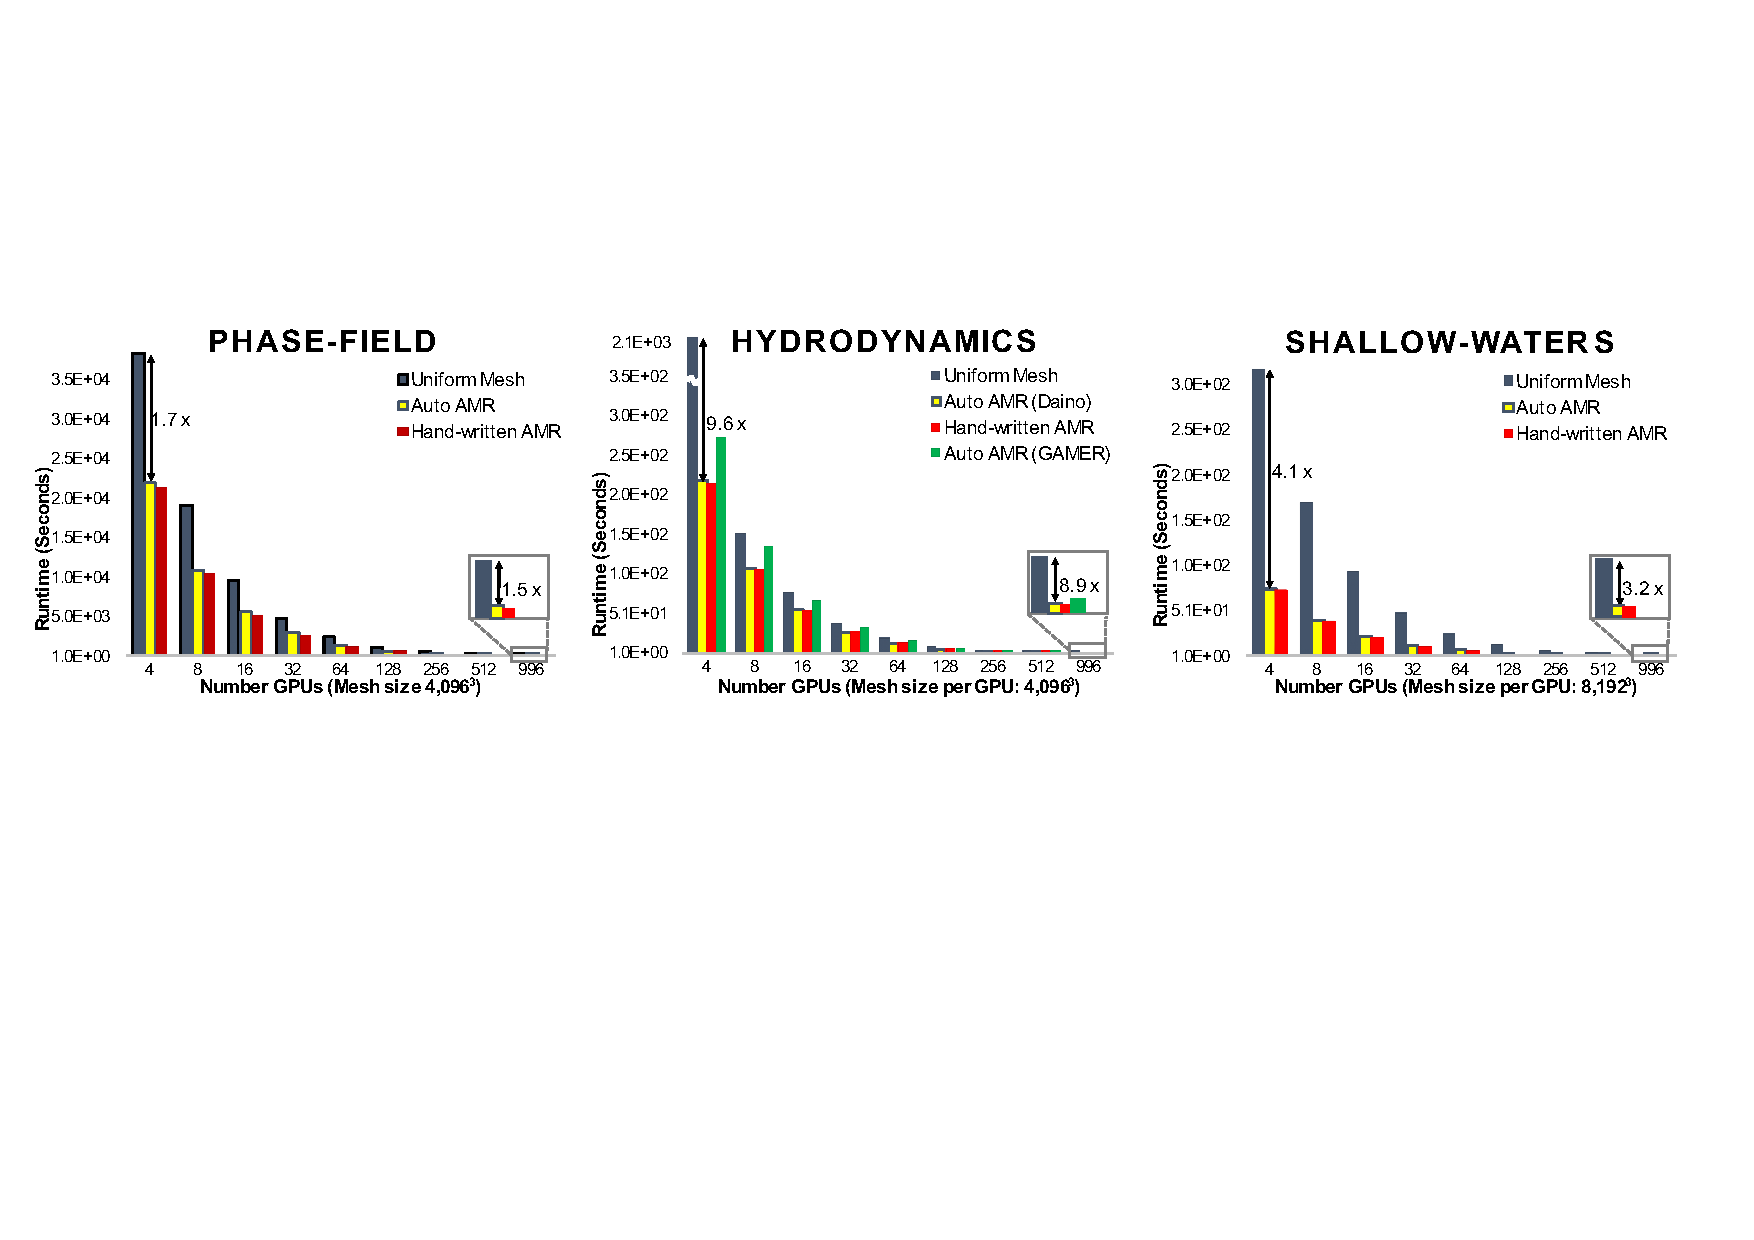
\includegraphics[width=\textwidth]{research/maruyama/wahib02.pdf}%1-expanded.pdf}%1.pdf}, 
%\caption{Strong scaling of hand-written AMR and Daino-generated AMR versus uniform mesh (Note: GAMER-generated AMR included in hydrodynamic solver)}
\caption{\small{Strong scaling of uniform mesh, hand-written and automated AMR (GAMER-generated AMR included in hydrodynamic)}}
 \locallabel{fig:wahib02}
%%\vspace{-5pt}
\end{figure*}

\textbf{Implementation:}
Our framework consists of a compiler and runtime components. We generate executables optimized for GPU execution by leveraging the LLVM compiler infrastructure. Our compiler builds on the LLVM compiler infrastructure. First, we use the front end to analyze and translate the stencil source code into GPU-optimized code in the form of LLVM Intermediate Representation (IR). Next, compiler passes are applied on the IR to add the AMR management code, which in turn make API calls to: a) the runtime API, and b) the GPU-optimized code generated by Nvidia back end code generator. Finally, LLVM IR is compiled and linked with the runtime libraries to generate an executable. The different stages of the compilation is managed by a shell script that the programmer invokes. 

We have built two libraries into the runtime. First, the \emph{AMR library} that encapsulates the AMR hierarchy management software. Second, the \emph{communication library} that wraps the MPI runtime library to simplify data movement operations for the AMR driver. 

\textbf{Applications:} We evalute our framework with three production applications. \emph{Phase-field simulation for dendritic growth}: We simulate 3D dendritic growth during solidification in a binary alloy using phase-field model. The computation requires a $2^{nd}$ order finite difference scheme for space with $1^{st}$ forward Euler-type finite difference method for time on a 3D uniform mesh. We use the code by Shimokawabe et. al as our reference implementation~\cite{Shimokawabe2011}. \emph{Hydrodynamics Solver}: We model a hydrodynamics application using 3D Euler equations. We explore a $2^{nd}$ order directionally split hyperbolic schemes to solve the equation. We use the code by GAMER framework for the Hydrodynamics solver as our reference implementation~\cite{Schive2012}. \emph{Shallow-water Solver}: We model shallow water simulations by depth-averaging the Navier--Stokes equations. We use a numerical method based on a semi-discrete, $2^{nd}$ order, central scheme. To advance the time step, we base our flux, max step, boundary condition, and time integration kernels on the model proposed by Saetra et. al~\cite{Saetra2015}.

\textbf{Experimental Setup:} We use the TSUBAME2.5 supercomputer at Tokyo Tech. Each node has two socket Intel Xeon X5670 2.93GHz CPUs (12 cores), and three Nvidia Kepler K20x GPUs with total 54GB and 18GB of system and GPU memory. The compute nodes are interconnected by dual QDR Infiniband networks with a full bisection-bandwidth fat-tree topology network. We use CUDA v7.0 Toolkit for GPU code and LLVM compiler infrastructure v3.8 for the framework. Single precision variables are adopted in all experiments for all applications. The hand-written and automated AMR versions of all applications use the data-centric AMR approach. All experiments used $16^3$ mesh block size and 2D CUDA thread blocks of size $16$x$16$ threads. All test runs are collected for $100,000$ time steps with a constant maximum of six refinement levels.

\textbf{Results:} In a weak scaling experiment, shown in Figure~\localref{fig:wahib01}, the runtime for uniform mesh, hand-written AMR, and auto-generated AMR are compared. The following points are important to note. First, more than $1.7$x speedup is achieved using our framework with $1000$ GPUs for the phase-field simulation. This is a considerable improvement considering that the uniform mesh implementation is a Gordon Bell prize winner for time-to-solution. Second, we included a comparison with the auto-generated AMR by GAMER framework for the hydrodynamics solver. The AMR code generated by our framework is faster than the code generated by GAMER, mainly because GAMER uses a pipeline to hide data movement latency while our framework uses a data-centric approach to avoid data movement altogether. Third, we achieve good scaling that is comparable to the scalability of the hand-written AMR code.

Figure~\localref{fig:wahib02} shows a strong scaling comparison for hand-written AMR and auto-generated AMR against uniform mesh implementation. The auto-generated AMR by our framework achieves runtime and scalability comparable to that of the uniform mesh implementation. However, when using more GPUs, reduction in speedup starts to occur as the management of AMR starts to dominate the simulation runtime. 
\subsection{High Performance Graph Analytics Study with Graph500}
% Maruyama

\section{Schedule and Future Plan}

\subsection{KMR}
% Takizawa & Matsuda

\subsection{High Level Framework for High Performance AMR}
% Wahib
Initially, we intend on testing expanding the framework to allow for user-defined boundary conditions and error estimation functions. We also intend on testing framework at larger scale using TSUBAME2.5 supercomputer (under a grant from JHPCN). Finally, we are closely working with collaborators on FLASH project at Chicago university (Dr. Anshu Dubey) to introduce an integration between our framework and FLASH

\subsection{High Performance Graph Analytics Study with Graph500}
% Maruyama

%%% DO NOT EDIT BELOW

\section{Publications}

%\printbibliography[keyword=journal, heading=subbibliography, title={Journal Articles}, prefixnumbers={1-}, resetnumbers=true]
%\printbibliography[keyword=proceedings, heading=subbibliography, title={Conference Papers}, prefixnumbers={2-}, resetnumbers=true]
%\printbibliography[keyword=invited, heading=subbibliography, title={Invited Talks}, prefixnumbers={3-}, resetnumbers=true]
%\printbibliography[keyword=poster, heading=subbibliography, title={Posters and Presentations}, prefixnumbers={4-}, resetnumbers=true]
%\printbibliography[keyword=deliverable, heading=subbibliography, title={Patents and Deliverables}, prefixnumbers={5-}, resetnumbers=true]

\printbibliography[keyword=journal, heading=subbibliography, title={Journal Articles}, resetnumbers=true]
\printbibliography[keyword=proceedings, heading=subbibliography, title={Conference Papers}]
\printbibliography[keyword=invited, heading=subbibliography, title={Invited Talks}]
\printbibliography[keyword=poster, heading=subbibliography, title={Posters and Presentations}]
\printbibliography[keyword=deliverable, heading=subbibliography, title={Patents and Deliverables}]

\end{refsection}
